\documentclass{article}
\title{Alle README's en code voorbereiding}

\usepackage{import}
\usepackage{hyperref}
\usepackage{pdfpages}
\usepackage{framed}
\usepackage{graphicx}
\usepackage{xcolor}
\usepackage{lmodern}
\usepackage{amssymb}
\usepackage{amsmath}
\PassOptionsToPackage{unicode=true}{hyperref} % options for packages loaded elsewhere
\PassOptionsToPackage{hyphens}{url}

\pdfstringdefDisableCommands{%
  \def\\{}%
  \def\newline{}%
  \def\texttt#1{<#1>}%
}

\newcounter{MarkdownId}

\usepackage{lmodern}
\usepackage{amssymb,amsmath}
\usepackage{ifxetex,ifluatex}
\ifnum 0\ifxetex 1\fi\ifluatex 1\fi=0 % if pdftex
  \usepackage[T1]{fontenc}
  \usepackage[utf8]{inputenc}
  \usepackage{textcomp} % provides euro and other symbols
\else % if luatex or xelatex
  \usepackage{unicode-math}
  \defaultfontfeatures{Ligatures=TeX,Scale=MatchLowercase}
\fi
% use upquote if available, for straight quotes in verbatim environments
\IfFileExists{upquote.sty}{\usepackage{upquote}}{}
% use microtype if available
\IfFileExists{microtype.sty}{%
\usepackage[]{microtype}
\UseMicrotypeSet[protrusion]{basicmath} % disable protrusion for tt fonts
}{}
\IfFileExists{parskip.sty}{%
\usepackage{parskip}
}{% else
\setlength{\parindent}{0pt}
\setlength{\parskip}{6pt plus 2pt minus 1pt}
}

\urlstyle{same}  % don't use monospace font for urls
\usepackage{color}
\usepackage{fancyvrb}
\newcommand{\VerbBar}{|}
\newcommand{\VERB}{\Verb[commandchars=\\\{\}]}
\DefineVerbatimEnvironment{Highlighting}{Verbatim}{commandchars=\\\{\}}
% Add ',fontsize=\small' for more characters per line
\newenvironment{Shaded}{}{}
\newcommand{\KeywordTok}[1]{\textcolor[rgb]{0.00,0.44,0.13}{\textbf{#1}}}
\newcommand{\DataTypeTok}[1]{\textcolor[rgb]{0.56,0.13,0.00}{#1}}
\newcommand{\DecValTok}[1]{\textcolor[rgb]{0.25,0.63,0.44}{#1}}
\newcommand{\BaseNTok}[1]{\textcolor[rgb]{0.25,0.63,0.44}{#1}}
\newcommand{\FloatTok}[1]{\textcolor[rgb]{0.25,0.63,0.44}{#1}}
\newcommand{\ConstantTok}[1]{\textcolor[rgb]{0.53,0.00,0.00}{#1}}
\newcommand{\CharTok}[1]{\textcolor[rgb]{0.25,0.44,0.63}{#1}}
\newcommand{\SpecialCharTok}[1]{\textcolor[rgb]{0.25,0.44,0.63}{#1}}
\newcommand{\StringTok}[1]{\textcolor[rgb]{0.25,0.44,0.63}{#1}}
\newcommand{\VerbatimStringTok}[1]{\textcolor[rgb]{0.25,0.44,0.63}{#1}}
\newcommand{\SpecialStringTok}[1]{\textcolor[rgb]{0.73,0.40,0.53}{#1}}
\newcommand{\ImportTok}[1]{#1}
\newcommand{\CommentTok}[1]{\textcolor[rgb]{0.38,0.63,0.69}{\textit{#1}}}
\newcommand{\DocumentationTok}[1]{\textcolor[rgb]{0.73,0.13,0.13}{\textit{#1}}}
\newcommand{\AnnotationTok}[1]{\textcolor[rgb]{0.38,0.63,0.69}{\textbf{\textit{#1}}}}
\newcommand{\CommentVarTok}[1]{\textcolor[rgb]{0.38,0.63,0.69}{\textbf{\textit{#1}}}}
\newcommand{\OtherTok}[1]{\textcolor[rgb]{0.00,0.44,0.13}{#1}}
\newcommand{\FunctionTok}[1]{\textcolor[rgb]{0.02,0.16,0.49}{#1}}
\newcommand{\VariableTok}[1]{\textcolor[rgb]{0.10,0.09,0.49}{#1}}
\newcommand{\ControlFlowTok}[1]{\textcolor[rgb]{0.00,0.44,0.13}{\textbf{#1}}}
\newcommand{\OperatorTok}[1]{\textcolor[rgb]{0.40,0.40,0.40}{#1}}
\newcommand{\BuiltInTok}[1]{#1}
\newcommand{\ExtensionTok}[1]{#1}
\newcommand{\PreprocessorTok}[1]{\textcolor[rgb]{0.74,0.48,0.00}{#1}}
\newcommand{\AttributeTok}[1]{\textcolor[rgb]{0.49,0.56,0.16}{#1}}
\newcommand{\RegionMarkerTok}[1]{#1}
\newcommand{\InformationTok}[1]{\textcolor[rgb]{0.38,0.63,0.69}{\textbf{\textit{#1}}}}
\newcommand{\WarningTok}[1]{\textcolor[rgb]{0.38,0.63,0.69}{\textbf{\textit{#1}}}}
\newcommand{\AlertTok}[1]{\textcolor[rgb]{1.00,0.00,0.00}{\textbf{#1}}}
\newcommand{\ErrorTok}[1]{\textcolor[rgb]{1.00,0.00,0.00}{\textbf{#1}}}
\newcommand{\NormalTok}[1]{#1}
\setlength{\emergencystretch}{3em}  % prevent overfull lines
\providecommand{\tightlist}{%
  \setlength{\itemsep}{0pt}\setlength{\parskip}{0pt}}

% set default figure placement to htbp
\makeatletter
\def\fps@figure{htbp}
\makeatother
% configure font
\usepackage[T1]{fontenc}
\usepackage{helvet}
% enable utf-8 symbols
\usepackage[utf8]{inputenc}

\usepackage{minted}

\begin{document}
    \maketitle

    \part{Voorbereide oefeningen}

    \hypertarget{bowling}{%
\section{Bowling}\label{bowling}}

Niet per se theoretisch moeilijk, maar veer regels met uitzonderingen
-\textgreater{} moeilijk om goed te krijgen.

    \inputminted{python}{../2011/bowling/oplossing.py3}

    \section{Achtbaan}
    \inputminted{python}{../2017/achtbaan/oplossing.py3}

    \section{Cluedo}
    \inputminted{python}{../2017/cluedo/oplossing.py3}

    \hypertarget{naomees}{%
\section{Naomees}\label{naomees}}

Simpele vraag met aan patern matching moet gedaan worden.

2 mogelijke oplossingsmethoden: * Handmatig gaan checken -\textgreater{}
\texttt{oplossing.py} * Converteer de taal naar regex -\textgreater{}
\texttt{alt\_oplossing.py}

Regex lijkt op het eerste zicht sneller omdat het intern versneld kan
worden, maar heeft het probleem met te algemeen te zijn.

Benchmarks:

\begin{Shaded}
\begin{Highlighting}[]
\ExtensionTok{$}\OperatorTok{\textgreater{}}\NormalTok{ hyperfine }\StringTok{"python alt\_oplossing.py \textless{}bench.input"} \StringTok{"python oplossing.py \textless{}bench.input"}
\ExtensionTok{Benchmark}\NormalTok{ 1: python alt\_oplossing.py }\OperatorTok{\textless{}}\NormalTok{bench.input}
  \ExtensionTok{Time} \ErrorTok{(}\ExtensionTok{mean}\NormalTok{ ± σ}\KeywordTok{)}\BuiltInTok{:}\NormalTok{      67.6 ms ±   8.4 ms    [User: 58.2 ms, System: 9.1 ms]}
  \ExtensionTok{Range} \ErrorTok{(}\ExtensionTok{min}\NormalTok{ … max}\KeywordTok{)}\BuiltInTok{:}\NormalTok{    55.9 ms …  88.3 ms    42 runs}
 
\ExtensionTok{Benchmark}\NormalTok{ 2: python oplossing.py }\OperatorTok{\textless{}}\NormalTok{bench.input}
  \ExtensionTok{Time} \ErrorTok{(}\ExtensionTok{mean}\NormalTok{ ± σ}\KeywordTok{)}\BuiltInTok{:}\NormalTok{      54.4 ms ±   8.9 ms    [User: 46.3 ms, System: 7.9 ms]}
  \ExtensionTok{Range} \ErrorTok{(}\ExtensionTok{min}\NormalTok{ … max}\KeywordTok{)}\BuiltInTok{:}\NormalTok{    41.8 ms …  70.3 ms    56 runs}
 
\ExtensionTok{Summary}
  \StringTok{\textquotesingle{}python oplossing.py \textless{}bench.input\textquotesingle{}}\NormalTok{ ran}
    \ExtensionTok{1.24}\NormalTok{ ± 0.26 times faster than }\StringTok{\textquotesingle{}python alt\_oplossing.py \textless{}bench.input\textquotesingle{}}
\end{Highlighting}
\end{Shaded}

    \inputminted{python}{../2017/naomees/oplossing.py3}

    \section{NightCrawler}
    \inputminted{python}{../2017/nightcrawler/oplossing.py3}
    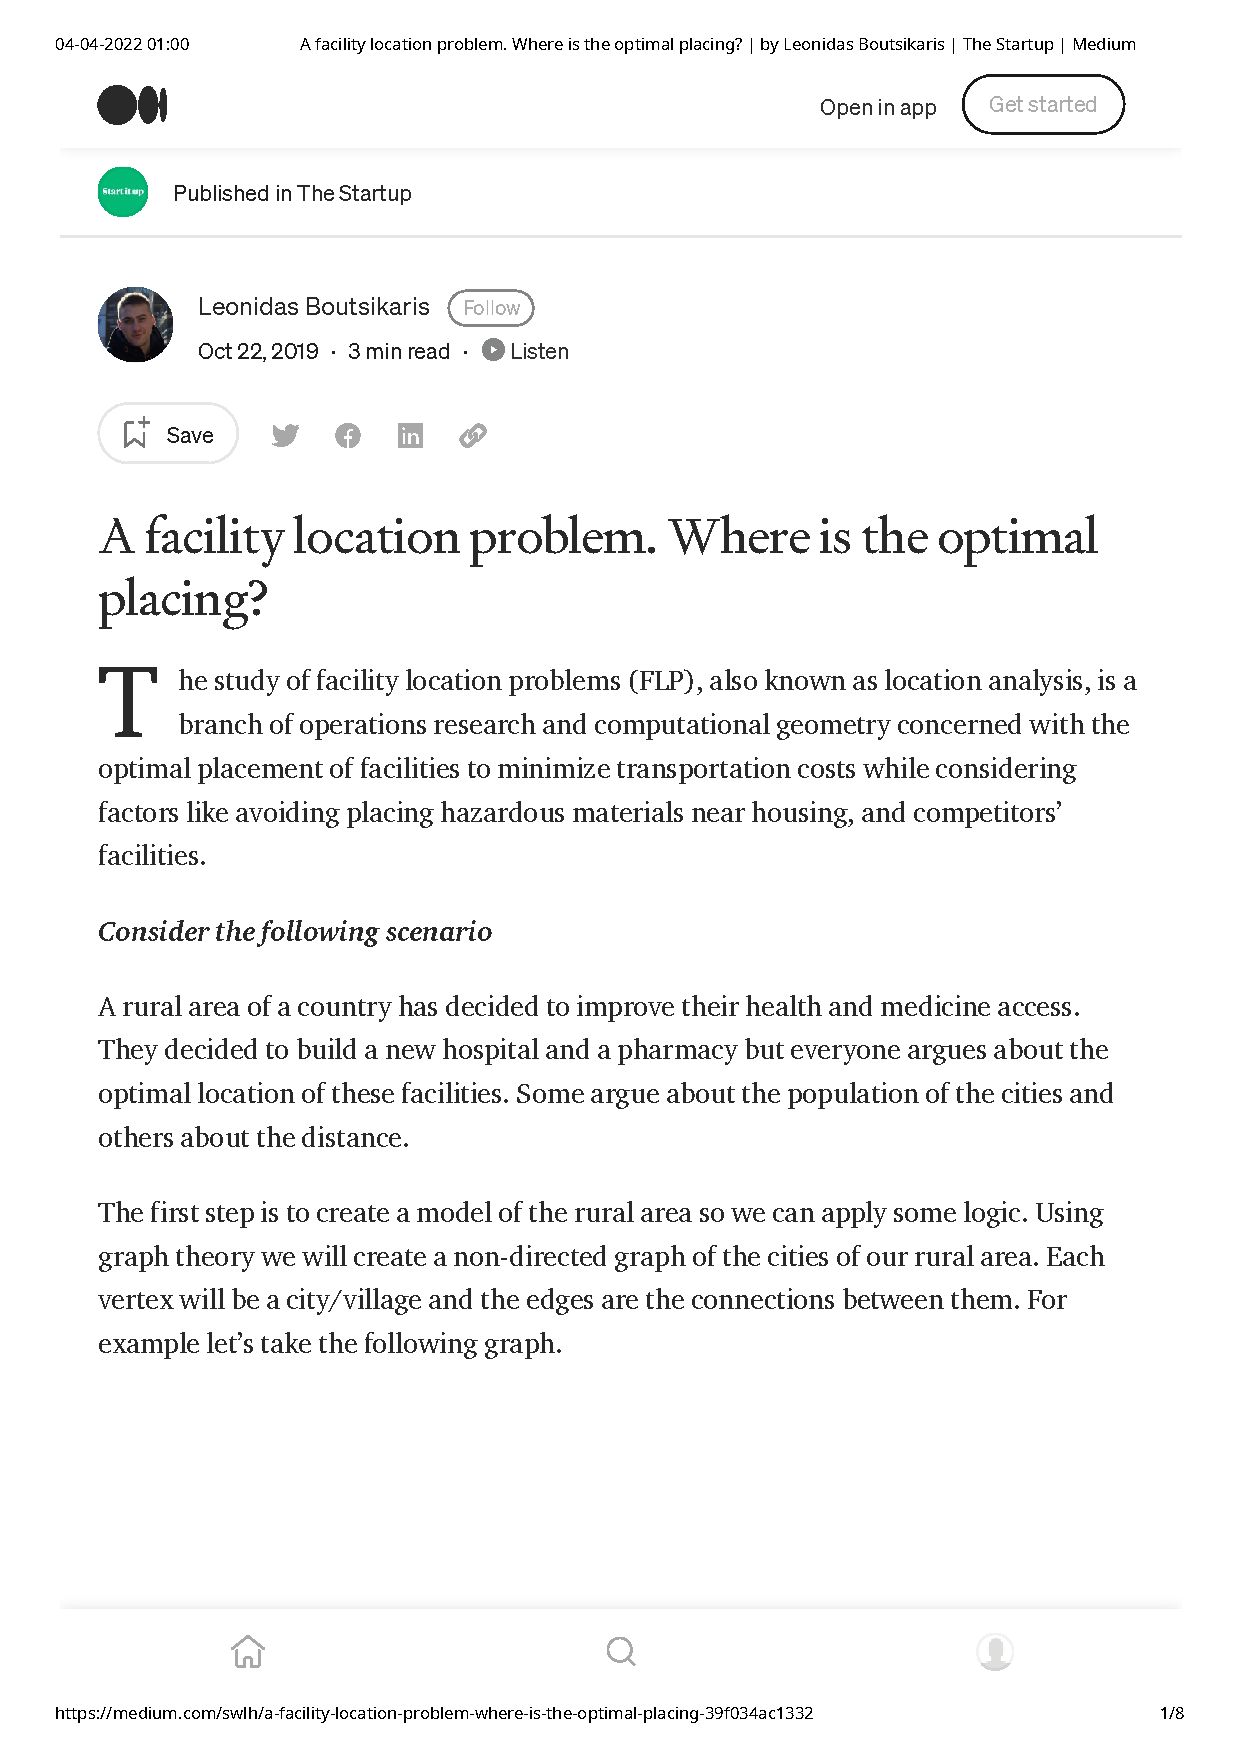
\includepdf[pages=-]{A facility location problem. Where is the optimal placing_ _ by Leonidas Boutsikaris _ The Startup _ Medium.pdf}

    \section{Bergwandeling}
    \inputminted{python}{../2018/bergwandeling/bergwandeling.py}

    \section{Buurland}
    \inputminted{python}{../2018/buurland/buurland.py}

    \section{Buurland (SamClercky)}
    \inputminted{python}{../2018/buurlanden_samclercky/oplossing.py3}

    \section{Slinger}
    \inputminted{python}{../2018/slinger/oplossing.py3}

    \hypertarget{beleefd}{%
\section{Beleefd}\label{beleefd}}

Programmeer technisch niet al te moeilijk. Moeilijk door wiskundige
theorie.

Interessante linken: * \url{https://nrich.maths.org/2074} *
\url{https://en.wikipedia.org/wiki/Polite_number}

Beleefd tot 20:

\begin{verbatim}
5 = 2 + ... + 3
6 = 1 + ... + 3
7 = 3 + ... + 4
9 = 2 + ... + 4
9 = 4 + ... + 5
10 = 1 + ... + 4
11 = 5 + ... + 6
12 = 3 + ... + 5
13 = 6 + ... + 7
14 = 2 + ... + 5
15 = 1 + ... + 5
15 = 4 + ... + 6
15 = 7 + ... + 8
17 = 8 + ... + 9
18 = 3 + ... + 6
18 = 5 + ... + 7
19 = 9 + ... + 10
20 = 2 + ... + 6
\end{verbatim}

\hypertarget{vinden-van-hoeveelheid-beleefde-nummers}{%
\subsection{Vinden van hoeveelheid beleefde
nummers}\label{vinden-van-hoeveelheid-beleefde-nummers}}

Het aantal oneven delers groter dat 1 = aantal te vinden sequenties

\hypertarget{aantal-sequenties}{%
\subsubsection{Aantal sequenties}\label{aantal-sequenties}}

\begin{enumerate}
\def\labelenumi{\arabic{enumi}.}
\tightlist
\item
  Decompositie in priem getallen
\item
  Neem de machten van de priemfactoren groter dan 1 en +1 voor elk
\item
  Vermenigvuldig alle en dan -1
\end{enumerate}

Vb. 90:

\begin{verbatim}
90 = 2 * 3^2 * 5^1
2,1 => (2+1) * (1+1) -1 = 5
\end{verbatim}

\hypertarget{constructie-sequentie}{%
\subsubsection{Constructie sequentie}\label{constructie-sequentie}}

\begin{Shaded}
\begin{Highlighting}[]
\CommentTok{\# x is totaal van som}
\CommentTok{\# y is oneven deler}
\NormalTok{x }\OperatorTok{=} \BuiltInTok{sum}\NormalTok{(i }\ControlFlowTok{for}\NormalTok{ i }\KeywordTok{in} \BuiltInTok{range}\NormalTok{(x}\OperatorTok{/}\NormalTok{y }\OperatorTok{{-}}\NormalTok{ (y}\OperatorTok{{-}}\DecValTok{1}\NormalTok{)}\OperatorTok{/}\DecValTok{2}\NormalTok{, x}\OperatorTok{/}\NormalTok{y }\OperatorTok{+}\NormalTok{ (y}\OperatorTok{+}\DecValTok{1}\NormalTok{)}\OperatorTok{/}\DecValTok{2}\OperatorTok{+}\DecValTok{1}\NormalTok{))}
\end{Highlighting}
\end{Shaded}

Het volstaat dus om enkel een priemfactorisatie te doen en de uiterste
te berekenen:

\begin{Shaded}
\begin{Highlighting}[]
\NormalTok{eerste }\OperatorTok{=}\NormalTok{ x}\OperatorTok{/}\NormalTok{y }\OperatorTok{{-}}\NormalTok{ (y}\OperatorTok{{-}}\DecValTok{1}\NormalTok{)}\OperatorTok{/}\DecValTok{2}
\NormalTok{laatste }\OperatorTok{=}\NormalTok{ x}\OperatorTok{/}\NormalTok{y }\OperatorTok{+}\NormalTok{ (y}\OperatorTok{+}\DecValTok{1}\NormalTok{)}\OperatorTok{/}\DecValTok{2}
\end{Highlighting}
\end{Shaded}

\begin{Shaded}
\begin{Highlighting}[]
\CommentTok{\# https://stackoverflow.com/questions/567222/simple{-}prime{-}number{-}generator{-}in{-}python}
\KeywordTok{def}\NormalTok{ is\_prime(num):}
    \ControlFlowTok{if}\NormalTok{ num }\OperatorTok{\textless{}} \DecValTok{2}\NormalTok{:         }\ControlFlowTok{return} \VariableTok{False}
    \ControlFlowTok{elif}\NormalTok{ num }\OperatorTok{\textless{}} \DecValTok{4}\NormalTok{:       }\ControlFlowTok{return} \VariableTok{True}
    \ControlFlowTok{elif} \KeywordTok{not}\NormalTok{ num }\OperatorTok{\%} \DecValTok{2}\NormalTok{:   }\ControlFlowTok{return} \VariableTok{False}
    \ControlFlowTok{elif}\NormalTok{ num }\OperatorTok{\textless{}} \DecValTok{9}\NormalTok{:       }\ControlFlowTok{return} \VariableTok{True}
    \ControlFlowTok{elif} \KeywordTok{not}\NormalTok{ num }\OperatorTok{\%} \DecValTok{3}\NormalTok{:   }\ControlFlowTok{return} \VariableTok{False}
    \ControlFlowTok{else}\NormalTok{:}
        \ControlFlowTok{for}\NormalTok{ n }\KeywordTok{in} \BuiltInTok{range}\NormalTok{(}\DecValTok{5}\NormalTok{, }\BuiltInTok{int}\NormalTok{(math.sqrt(num) }\OperatorTok{+} \DecValTok{1}\NormalTok{), }\DecValTok{6}\NormalTok{):}
            \ControlFlowTok{if} \KeywordTok{not}\NormalTok{ num }\OperatorTok{\%}\NormalTok{ n:}
                \ControlFlowTok{return} \VariableTok{False}
            \ControlFlowTok{elif} \KeywordTok{not}\NormalTok{ num }\OperatorTok{\%}\NormalTok{ (n }\OperatorTok{+} \DecValTok{2}\NormalTok{):}
                \ControlFlowTok{return} \VariableTok{False}

    \ControlFlowTok{return} \VariableTok{True}
\end{Highlighting}
\end{Shaded}

    \inputminted{python}{../2021/beleefd/oplossing.py3}
    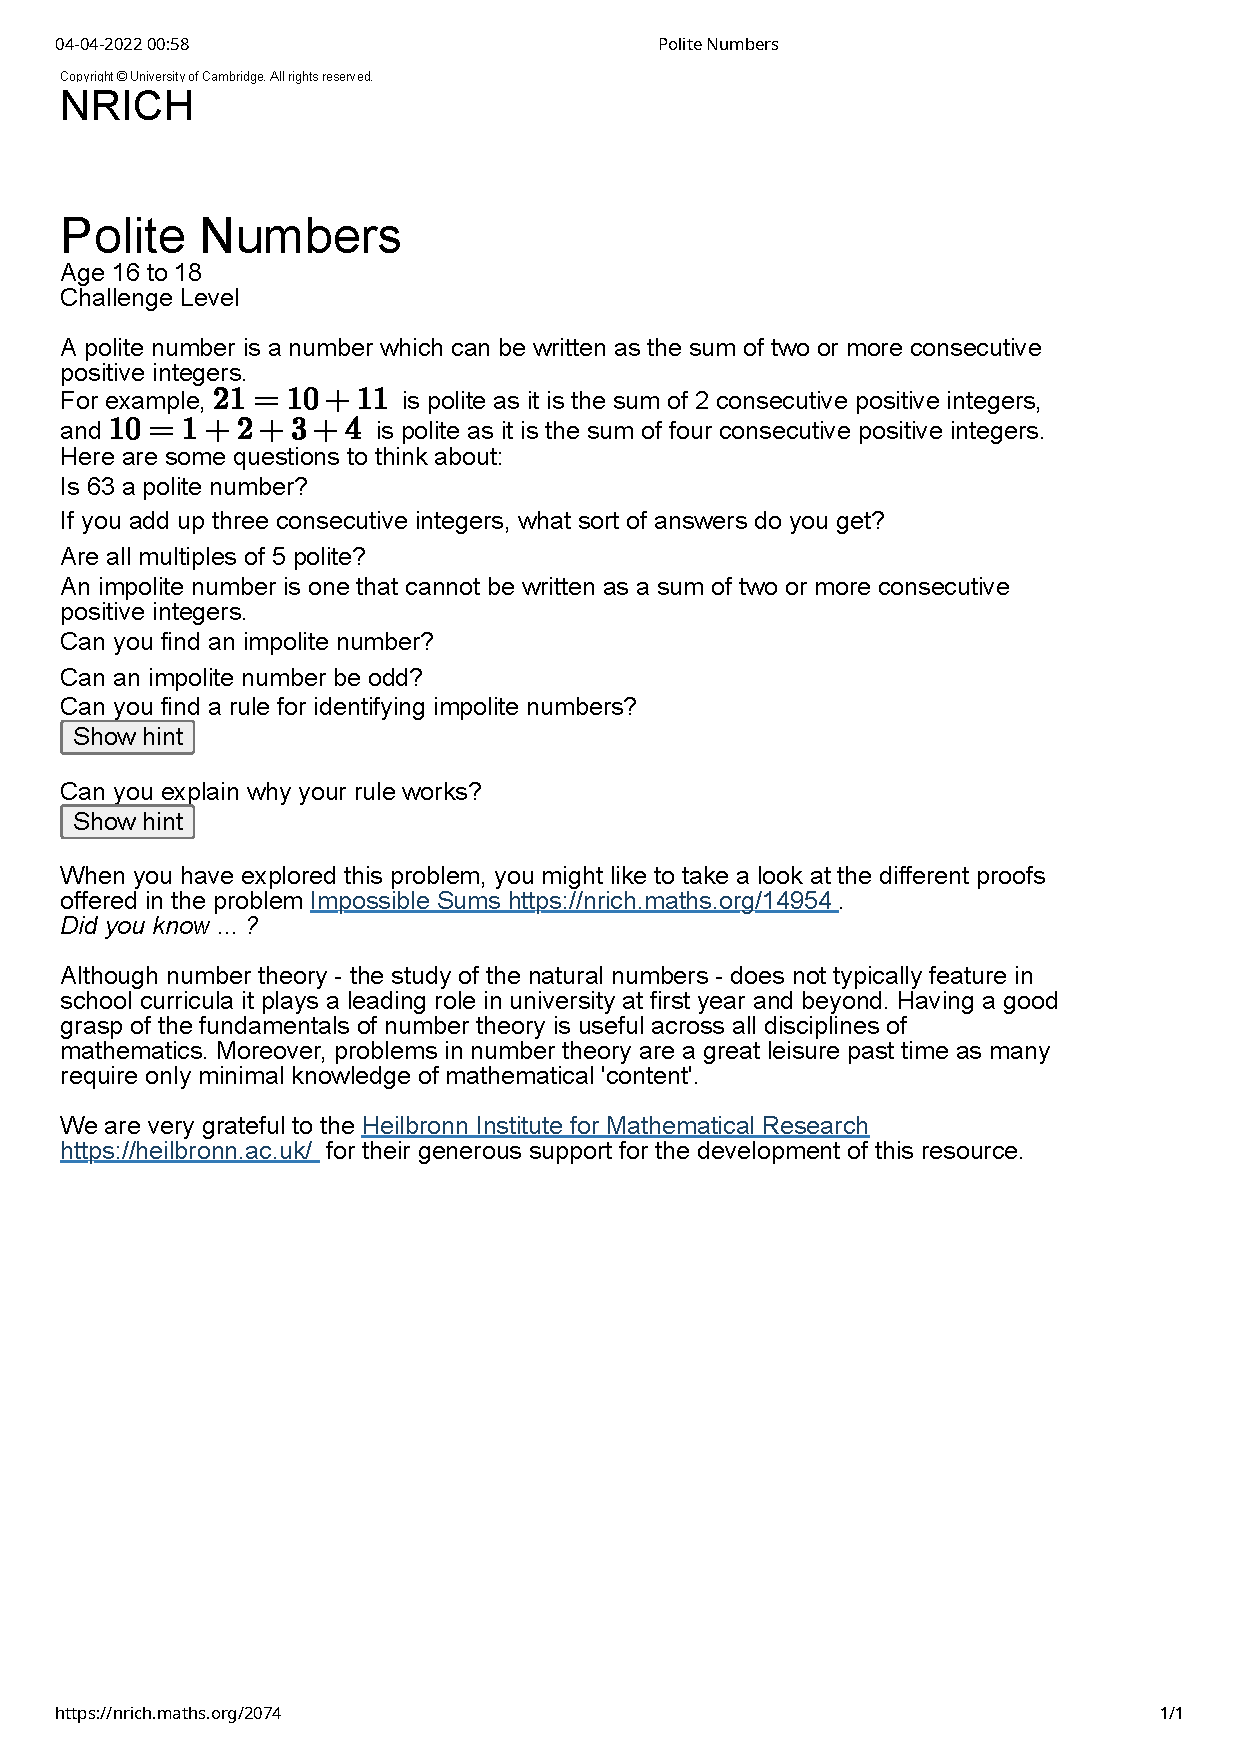
\includepdf[pages=-]{Polite Numbers.pdf}
    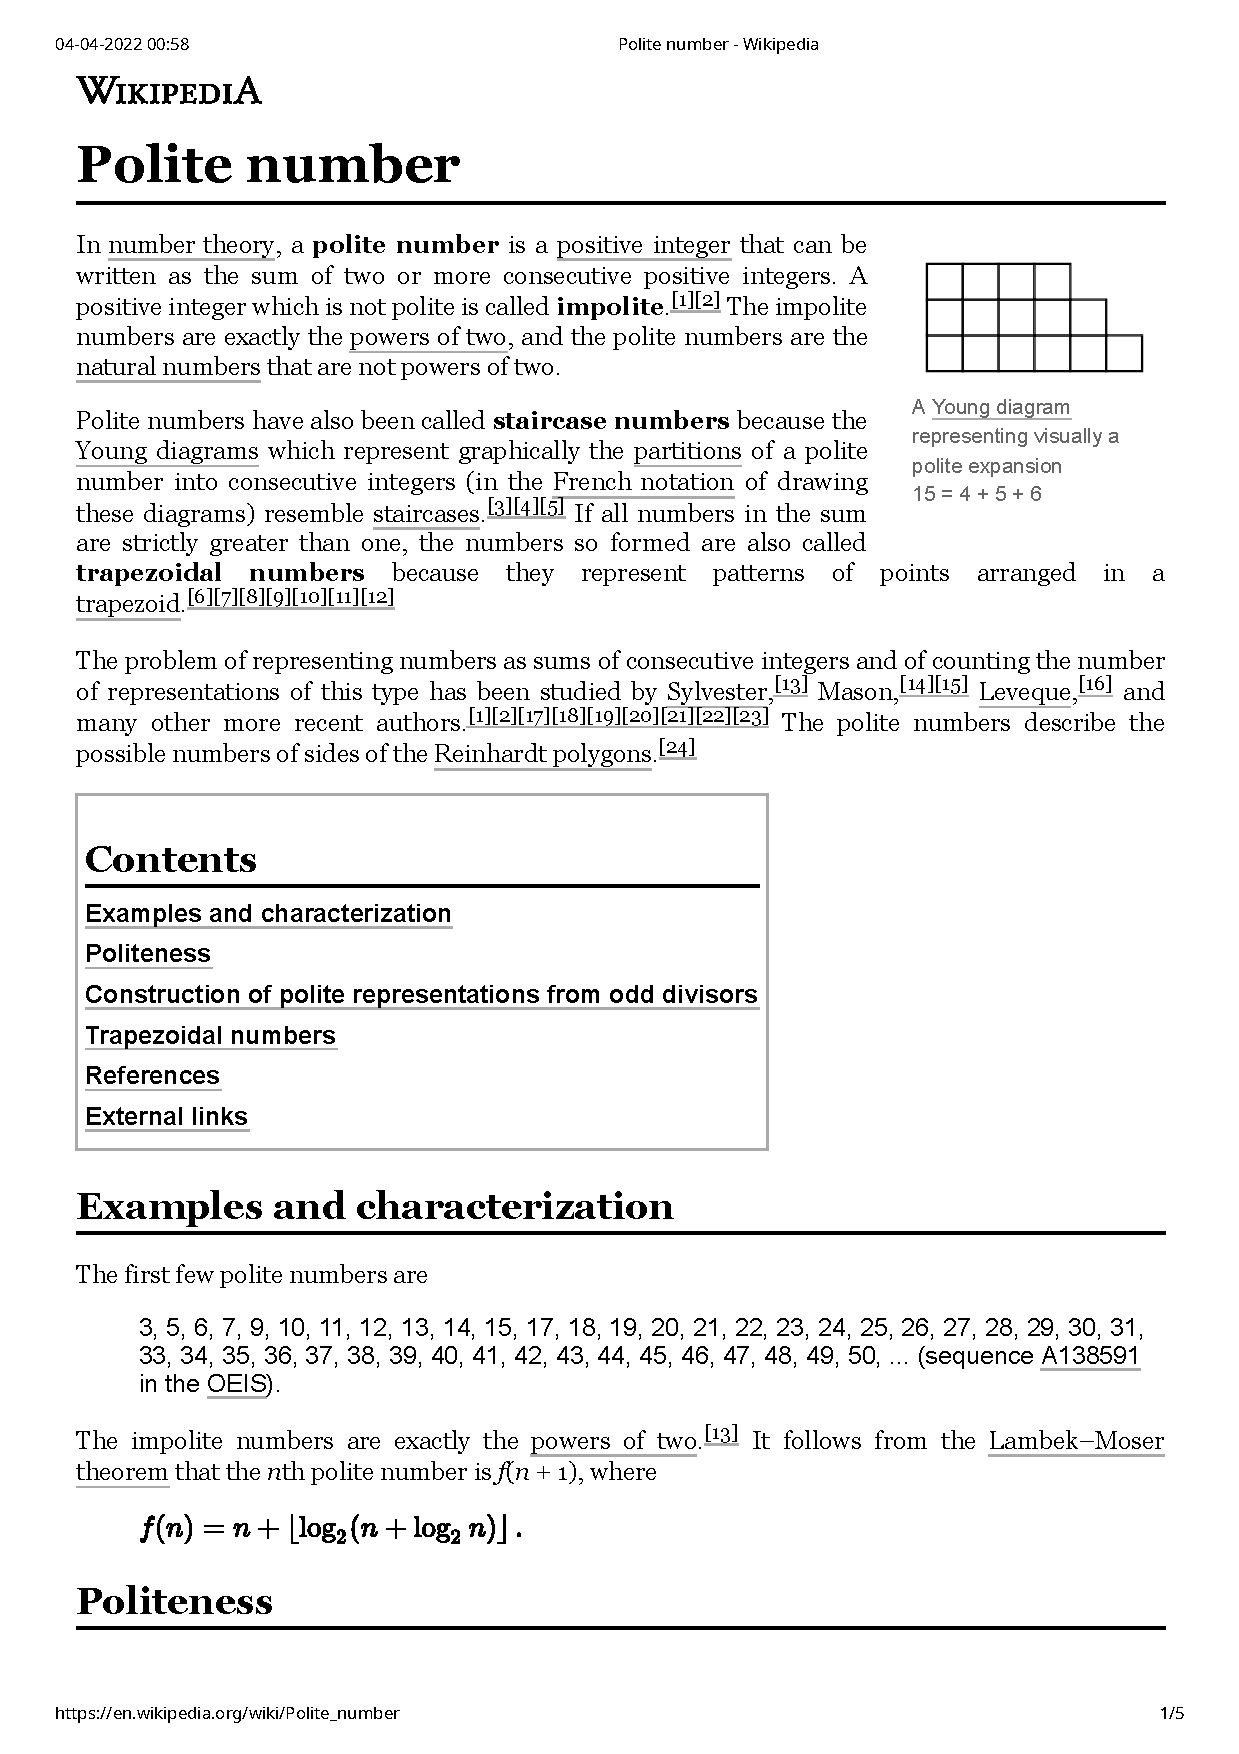
\includepdf[pages=-]{Polite number - Wikipedia.pdf}

    \hypertarget{regels-afbreken}{%
\section{Regels afbreken}\label{regels-afbreken}}

\hypertarget{formule-rafeligheid}{%
\subsection{Formule rafeligheid}\label{formule-rafeligheid}}

\begin{Shaded}
\begin{Highlighting}[]
\NormalTok{lines }\OperatorTok{=}\NormalTok{ [}\StringTok{"Lijn 1 tekst"}\NormalTok{, }\StringTok{"Lijn 2 tekst"}\NormalTok{]}
\NormalTok{max\_len\_regel }\OperatorTok{=} \BuiltInTok{max}\NormalTok{(}\BuiltInTok{len}\NormalTok{(line) }\ControlFlowTok{for}\NormalTok{ line }\KeywordTok{in}\NormalTok{ lines)}
\NormalTok{rafel }\OperatorTok{=} \BuiltInTok{sum}\NormalTok{((max\_len\_regel }\OperatorTok{{-}} \BuiltInTok{len}\NormalTok{(line)}\OperatorTok{**}\DecValTok{2} \ControlFlowTok{for}\NormalTok{ line }\KeywordTok{in}\NormalTok{ lines))}
\end{Highlighting}
\end{Shaded}

\hypertarget{constructie-met-minimale-rafeligheid}{%
\subsection{Constructie met minimale
rafeligheid}\label{constructie-met-minimale-rafeligheid}}

\begin{Shaded}
\begin{Highlighting}[]
\NormalTok{max\_len }\OperatorTok{=} \DecValTok{80}
\NormalTok{input\_text }\OperatorTok{=} \StringTok{"bla bla bla bla bla"}
\NormalTok{input\_len }\OperatorTok{=} \BuiltInTok{len}\NormalTok{(input\_text)}
\NormalTok{result }\OperatorTok{=}\NormalTok{ []}
\NormalTok{index }\OperatorTok{=} \DecValTok{0}
\ControlFlowTok{while}\NormalTok{ index }\OperatorTok{\textless{}}\NormalTok{ input\_len:}
\NormalTok{    start\_index }\OperatorTok{=}\NormalTok{ index}
    \CommentTok{\# advance max\_len}
\NormalTok{    index }\OperatorTok{+=} \DecValTok{80}
    \ControlFlowTok{if}\NormalTok{ index }\OperatorTok{\textless{}}\NormalTok{ input\_len:}
        \CommentTok{\# backtrack to prev whitespace}
        \ControlFlowTok{while}\NormalTok{ input\_text[index] }\OperatorTok{!=} \StringTok{" "}\NormalTok{:}
\NormalTok{            index }\OperatorTok{{-}=} \DecValTok{1}
\NormalTok{        result.append(input\_text[start\_index:index])}
\end{Highlighting}
\end{Shaded}

Opm: Het is waarschijnlijk mogelijk om de maximum en lengte van alle
aparte onderdelen te berekenen in vorig stuk code. Er wordt niet
gevraagd naar de geformateerde tekst, enkel de rafeligheid!


    \section{Minmax}
    \inputminted{python}{../2022/minmax/oplossing.py3}

    \part{Python documentatie}
    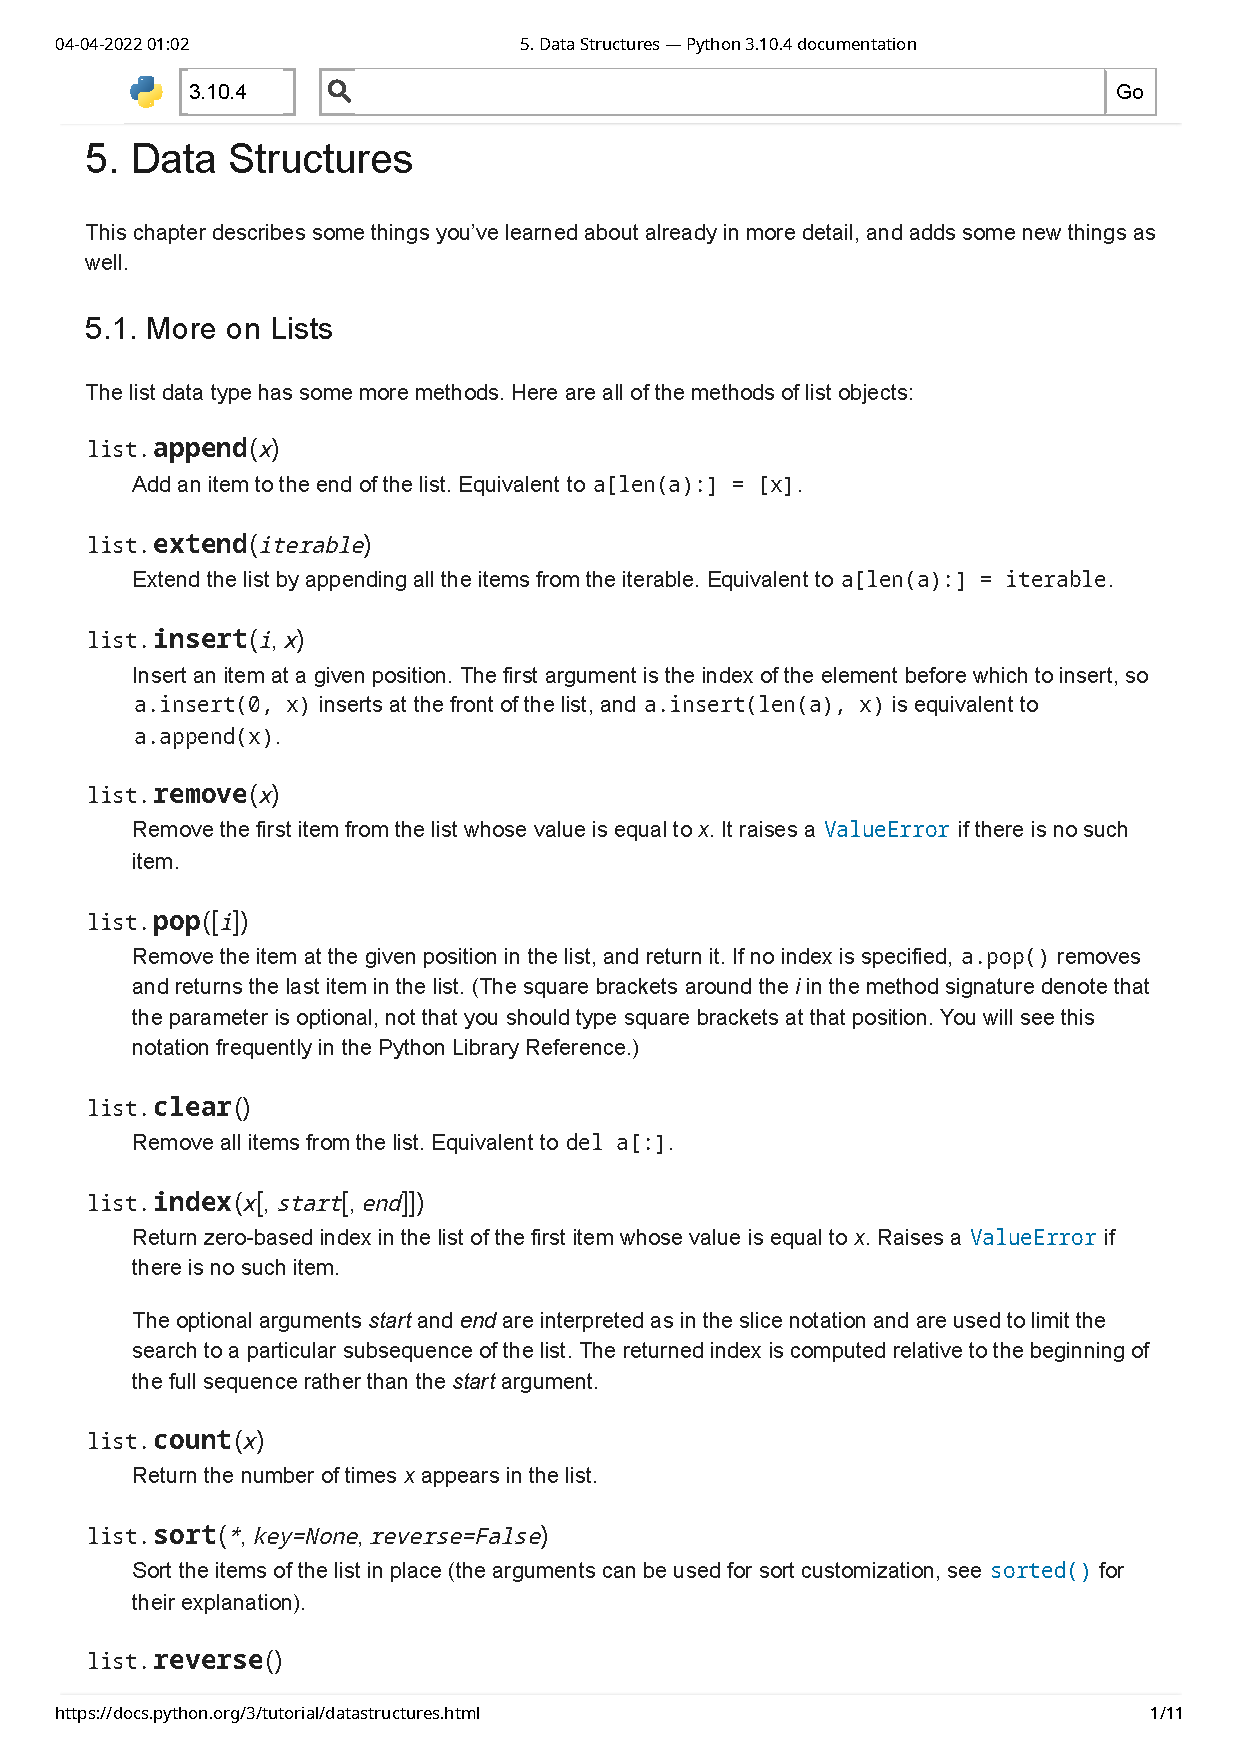
\includepdf[pages=-]{python-dict.pdf}
    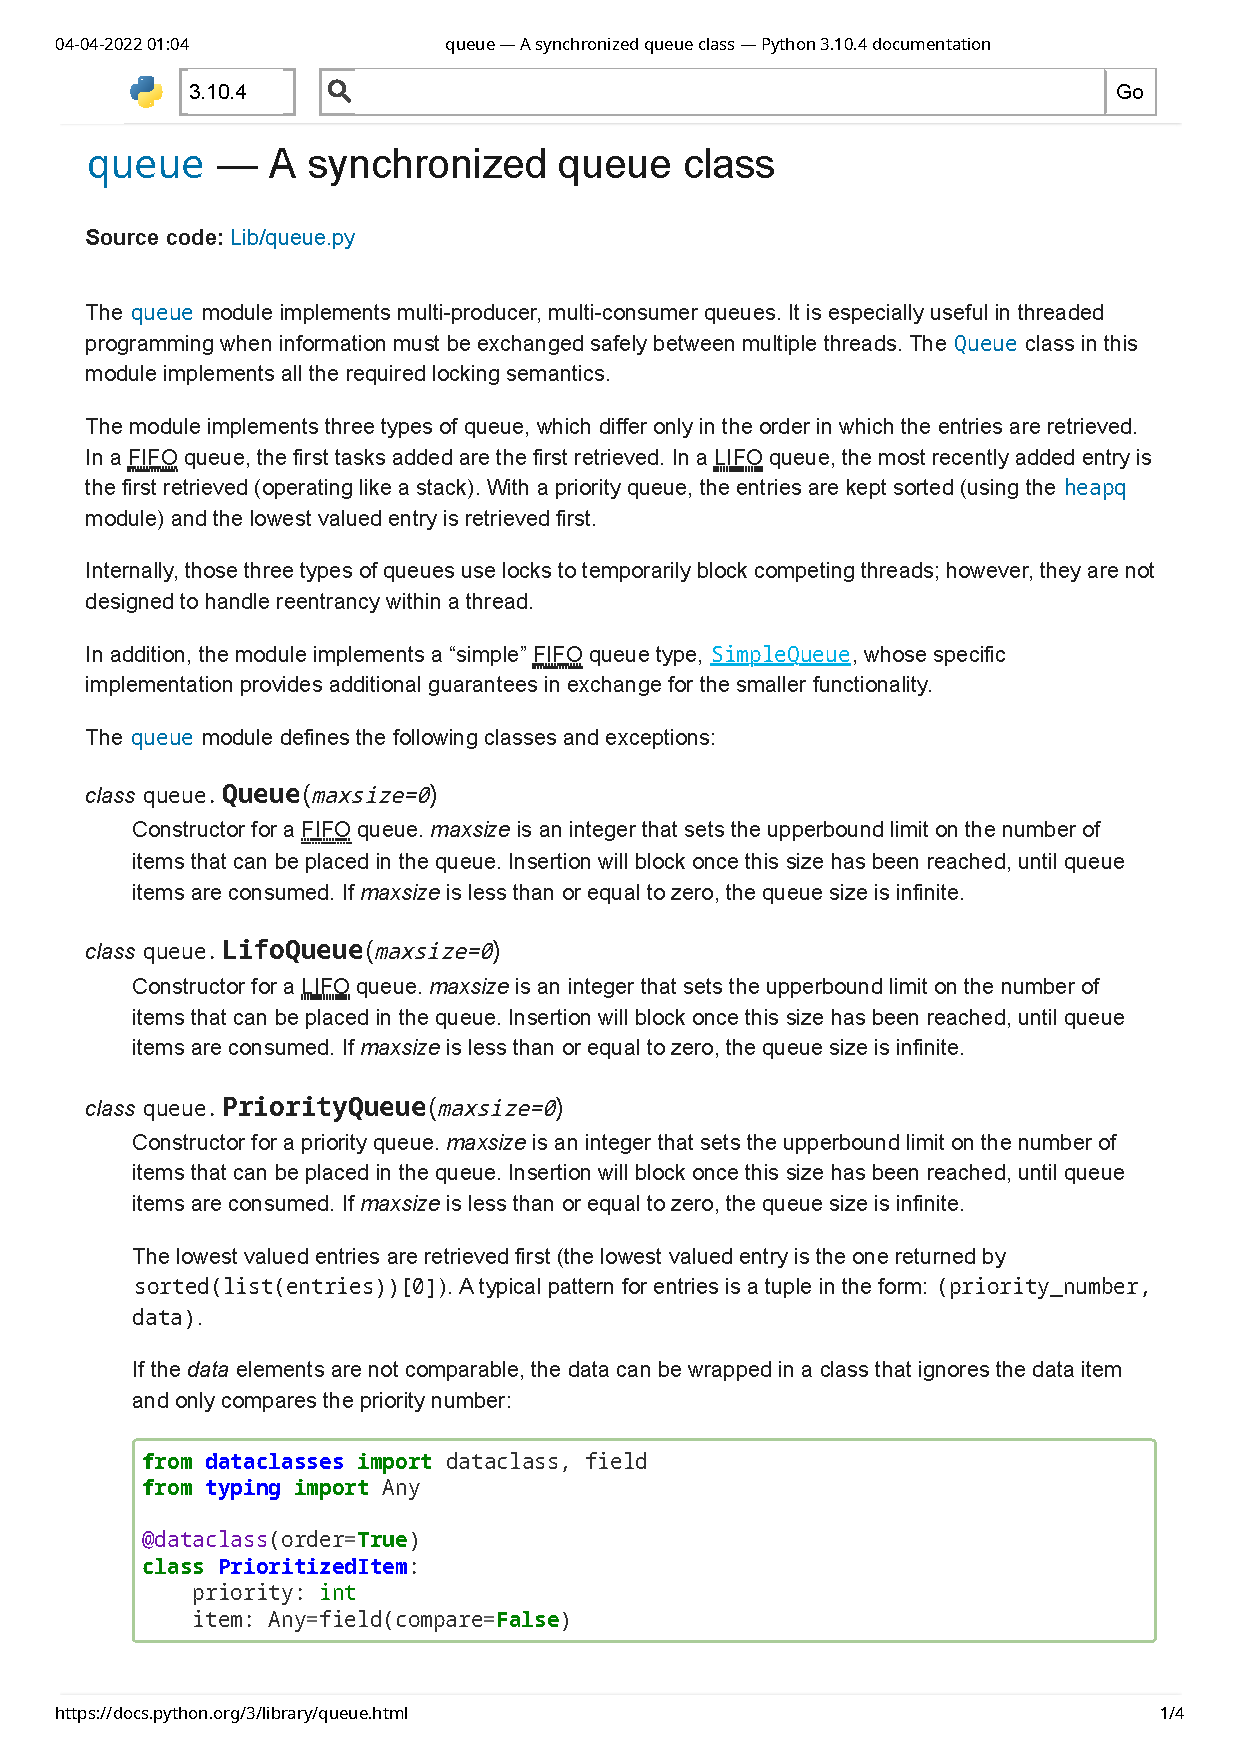
\includepdf[pages=-]{python-queue.pdf}

\end{document}
